\documentclass[12pt]{article}
\usepackage[czech]{babel}
\usepackage[utf8]{inputenc}
\usepackage[T1]{fontenc}
\usepackage{fullpage}
\usepackage{graphicx}
\renewcommand{\baselinestretch}{1.3}

\begin{document}
\section{Mechanické složení}
Konstrukce z Merkuru. Držák na sensor čáry vytištěn na 3D tiskárně. Držák na ultrazvukové sensory ze dřeva. Veškeré komponenty jsou k hlavní desce propojeny přes ploché nakrimpované kabely. Baterie připojena na svorkovnici, ze které vede kabel na spínač a následně do svorkovnice na hlavní desce. Hlavní deska s Arduinem je uchycena vzhůru nohama uprostřed robota pro lepší rozložení hmotnosti.

\section{Elektrická část}
Všechna propojení a připojení jsou na hlavní univerzální desce.
\begin{figure}[h]
	\centering
	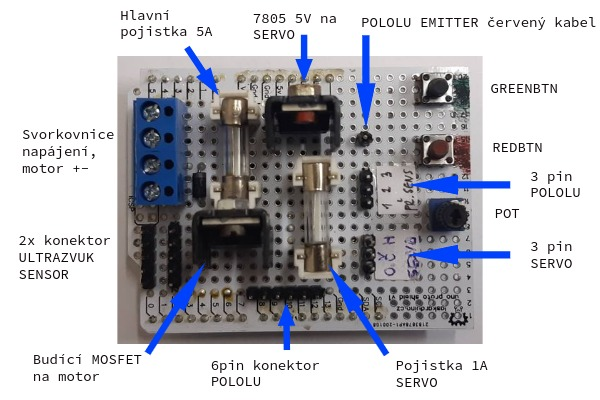
\includegraphics[scale=0.15]{deska.jpg}	
	\caption{Hlavní elektrická deska}
	\label{1}
\end{figure}
\end{document}
